\documentclass{amsart}
\usepackage[utf8]{inputenc}

\usepackage{amsmath, amssymb, amsthm}
\usepackage{enumitem}
\usepackage{hyperref}
\usepackage{float}
\usepackage{tikz}

\usepackage{listings}
\usepackage{xcolor}

\definecolor{bluekeywords}{rgb}{0.13, 0.19, 0.7}
\definecolor{goldenkeywords}{rgb}{0.67, 0.58, 0.13}
\definecolor{greencomments}{rgb}{0.1, 0.5, 0.2}
\definecolor{redstrings}{rgb}{0.8, 0.15, 0.1}
\definecolor{graynumbers}{rgb}{0.5, 0.5, 0.5}
\definecolor{subtlegray}{rgb}{0.98, 0.98, 0.98}

\usepackage{lstautogobble}
\usepackage{listings}

\lstset{
    autogobble,    
    columns=fullflexible,
    showspaces=false,
    showtabs=false,
    breaklines=true,
    showstringspaces=false,
    breakatwhitespace=true,
    escapeinside={(*@}{@*)},
    rulecolor=\color{lightgray},
    backgroundcolor=\color{subtlegray},
    commentstyle=\color{greencomments},
    keywordstyle=\color{bluekeywords},
    ndkeywordstyle=\color{goldenkeywords},
    stringstyle=\color{redstrings},
    numberstyle=\color{graynumbers},
    basicstyle=\ttfamily\linespread{1.15}\footnotesize,
    frame=tb,
    framesep=12pt,
    framexleftmargin=12pt,
    tabsize=4,
    captionpos=b
}

\lstdefinelanguage{TML}{ 
    keywords={changeto, move, goto, if, switch, while, module, accept, reject, halt, alphabet},
    ndkeywords={left, right, tapehead, blank},
    sensitive=true,
    comment=[l]{//},
    morecomment=[s]{/*}{*/},
    morestring=[b]',
    morestring=[b]"
}

\newtheorem{theorem}{Theorem}[section]
\theoremstyle{definition}
\newtheorem{definition}[theorem]{Definition}
\newtheorem{remark}[theorem]{Remark}
\newtheorem{example}[theorem]{Example}

\title{TML Equivalence Proof}
\author[P. Gautam]{Pete Gautam}

\begin{document}

    \begin{abstract}
        This document proves the equivalence of the TML with TMs. We do this by constructing an equivalent TML program for a TM, and vice versa. In the first section, we define complete TML programs, which are very close to TMs, and describe how they can be mapped into TMs.  In the second section, we define formally how complete TML programs can be transformed into TMs, and vice versa. Finally, the third section describes how we can transform a valid TML program into a complete TML program.
    \end{abstract}    
    \maketitle

    \section{Complete TML programs}
    \noindent Complete programs in the TML are a specific type of TML programs that are very detailed and obey different properties. As such, it is very easy to construct the TM corresponding to a complete program. In this section, we will build to the definition complete programs from complete blocks and modules.
    \begin{definition}
        Let $P$ be a valid TML program, and let $B$ be a basic block in $P$. We say that $B$ is a \emph{complete block} if it is composed of all the 3 commands: a \textit{changeto} command, a \textit{move} command, and a \textit{flow} command. If the \textit{flow} command is missing, we say that $B$ is a \emph{partially complete block}.
    \end{definition}

    Complete blocks contain all the information required to transition from one state to another. This is because of the following:
    \begin{itemize}
        \item A complete block lists the next value of the tapehead; we assume the original value of the tapehead to be known outwith the block.
        \item A complete block states which direction the tapehead is moving- left or right.
        \item A complete block determines precisely what the next state is for the block- it is either a terminating state or we are going to the initial block of another module.
    \end{itemize}        
    We can convert any basic block with a \textit{flow} command to a complete block by adding the default commands (i.e. moving left and changing the tapehead value to the current value). Equally, it is quite straightforward to convert a complete block into a subpart of a Turing Machine.
    \begin{example}
        Consider the following complete block.
\begin{lstlisting}[language=TML]
changeto a
move right
goto s2
\end{lstlisting}
        \noindent If we are at the state $s_1$, and the block applies when the tapehead value is $b$, then the following is the corresponding subpart of the Turing Machine:
        \begin{figure}[H]
            \centering
            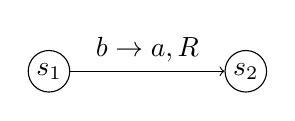
\begin{tikzpicture}
                \node[circle, draw=black, fill=white, inner sep=0pt, minimum size=15pt] (s1) at (0, 0) {$s_1$};
                \node[circle, draw=black, fill=white, inner sep=0pt, minimum size=15pt] (s2) at (2.5, 0) {$s_2$};
    
                \draw[->] (s1) -- node[above] {$b \to a, R$} (s2);
            \end{tikzpicture}
            \caption{The TM subpart of the given Turing Machine complete block.}
        \end{figure}            
    \end{example}
    
    Using complete and partially complete blocks, we can define complete modules.
    \begin{definition}
        Let $P$ be a valid TML program, and let $M$ be a module in $P$. We say that $M$ is a \emph{complete module} if all of the following hold:
        \begin{itemize}
            \item it is composed of a single switch block;
            \item the body of each \textit{if} command is a complete block; and
            \item the body of each \textit{while} command is a partially complete block.
        \end{itemize}
    \end{definition}

    % \begin{remark}
    %     Having no \textit{if} commands in a complete module means that the Turing machine never terminates. This is not an issue since it is still a valid Turing machine. 
    % \end{remark}
    
    \begin{remark}
        For a \textit{while} command, the body must be partially complete because the corresponding edge in the TM is always a loop.
    \end{remark}
    
    It is quite easy to map a single module to a sub-Turing machine. It precisely corresponds to having an initial state and edges going to other states as dictated by each case. Because the program is valid, we know that there is a case for each letter in the alphabet, including the \texttt{blank} letter.
    \begin{example}
        Consider the following complete module.
\begin{lstlisting}[language=TML]
module basic {
    switch tapehead {
        while b {
            changeto b
            move right
        } if a, blank {
            changeto blank
            move left
            reject
        }
    }
}
\end{lstlisting}
    If the alphabet is composed only of $a$ and $b$, then the corresponding sub-TM is the following:
    \begin{figure}[H]
        \centering
        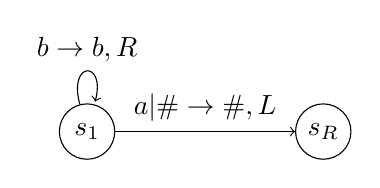
\begin{tikzpicture}
            \node[circle, draw=black, fill=white, inner sep=0pt, minimum size=20pt] (s1) at (0, 0) {$s_1$};
            \node[circle, draw=black, fill=white, inner sep=0pt, minimum size=20pt] (sR) at (3, 0) {$s_R$};

            \draw[->] (s1) -- node[above] {$a | \# \to \#, L$} (sR);
            \draw[->] (s1) edge[loop above] node[above] {$b \to b, R$} (s1);
        \end{tikzpicture}
        \caption{The sub-TM of the given Turing Machine complete module.}
    \end{figure}
    \end{example}

    \begin{remark}
        In the example above, we consider the state $s_1$ to be the \emph{corresponding state} of the module. For every complete module, there is precisely one corresponding state.
    \end{remark}

    Now, we can define complete programs.
    \begin{definition}
        Let $P$ be a TML program. We say that $P$ is \emph{complete} if it is composed of one or more complete modules. We also require every \textit{goto} command in a complete block to refer to an existing module.
    \end{definition}

    \begin{remark}
        The second condition (called \emph{valid reference}) is required for any TML program.
    \end{remark}

    \begin{remark}
        In general, a complete program is not composed of a single complete module. We will see later that a relatively simple module can be broken down into a couple of complete modules, each of which refer to each other.
    \end{remark}
    
    Every module in the program can be converted to a state, along with directed edges to other states. If the program is complete, then we ensure that the states connect to form a valid TM.
    
    \begin{example}
        Consider the following complete program.
\begin{lstlisting}[language=TML]
alphabet = {"a", "b"}
module isDivTwo {
    switch tapehead {
        while 0 {
            changeto 0
            move right
        } while 1 {
            changeto 1
            move right
        } if blank {
            changeto blank
            move left
            goto isDivTwoCheck
        }
    }
}
module isDivTwoCheck {
    switch tapehead {
        if 0 {
            changeto 0
            move left
            accept
        } if 1, blank {
            changeto blank
            move left
            reject
        }
    }
}
\end{lstlisting}
    Then, the corresponding TM is the following:
    \begin{figure}[H]
        \centering
        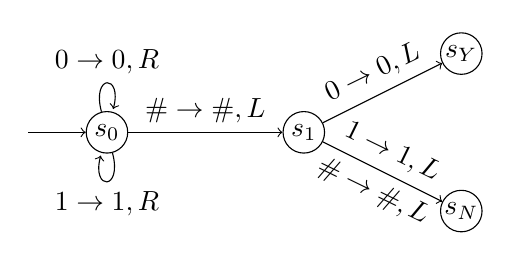
\begin{tikzpicture}
            \node[circle, draw=black, fill=white, inner sep=0pt, minimum size=15pt] (s0) at (0, 0) {$s_0$};
            \node[circle, draw=black, fill=white, inner sep=0pt, minimum size=15pt] (s1) at (2.5, 0) {$s_1$};
            \node[circle, draw=black, fill=white, inner sep=0pt, minimum size=15pt] (sY) at (4.5, 1) {$s_Y$};
            \node[circle, draw=black, fill=white, inner sep=0pt, minimum size=15pt] (sN) at (4.5, -1) {$s_N$};
            
            \draw[->] (-1, 0) -- (s0);
            \draw[->] (s0) edge[loop above] node[above] {$0 \to 0, R$} (s0);
            \draw[->] (s0) edge[loop below] node[below] {$1 \to 1, R$} (s0);
            \draw[->] (s0) -- node[above] {$\# \to \#, L$} (s1);
            \draw[->] (s1) -- node[above, rotate=26] {$0 \to 0, L$} (sY);
            \draw[->] (s1) -- node[above, rotate=-26] {$1 \to 1, L$} node[below, rotate=-26] {$\# \to \#, L$} (sN);
        \end{tikzpicture}
        \caption{The TM of the given TML program. The state $s_0$ corresponds to the module \texttt{isDivTwo} and the state $s_1$ corresponds to the module \texttt{isDivTwoCheck}.}
    \end{figure}
    \end{example}
    
    \begin{remark}
        In the example above, we converted a complete TML program into a TM. It is equally possible to convert a TM into a complete TML program.
    \end{remark}

    \begin{example}
        Consider the following TM:
        \begin{figure}[H]
            \centering
            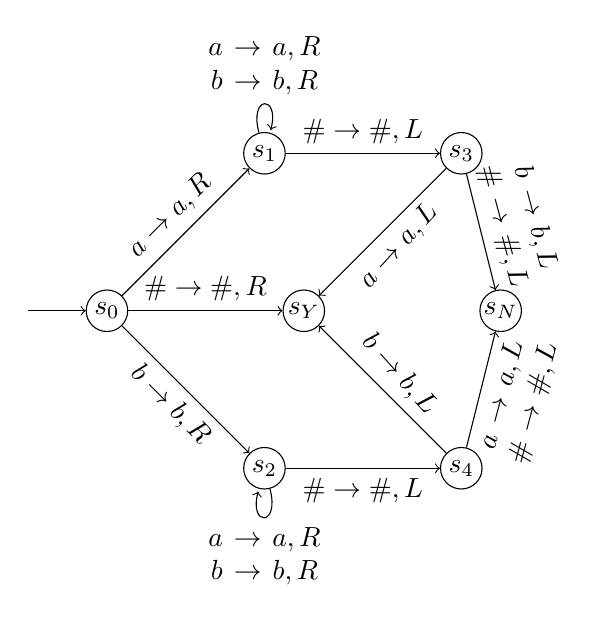
\begin{tikzpicture}
                \node[circle, draw=black, fill=white, inner sep=0pt, minimum size=15pt] (s0) at (0, 0) {$s_0$};
                \node[circle, draw=black, fill=white, inner sep=0pt, minimum size=15pt] (s1) at (2, 2) {$s_1$};
                \node[circle, draw=black, fill=white, inner sep=0pt, minimum size=15pt] (s2) at (2, -2) {$s_2$};
                \node[circle, draw=black, fill=white, inner sep=0pt, minimum size=15pt] (s3) at (4.5, 2) {$s_3$};
                \node[circle, draw=black, fill=white, inner sep=0pt, minimum size=15pt] (s4) at (4.5, -2) {$s_4$};
                \node[circle, draw=black, fill=white, inner sep=0pt, minimum size=15pt] (sY) at (2.5, 0) {$s_Y$};
                \node[circle, draw=black, fill=white, inner sep=0pt, minimum size=15pt] (sN) at (5, 0) {$s_N$};
                
                \draw[->] (-1, 0) -- (s0);
                \draw[->] (s0) -- node[above, rotate=45] {$a \to a, R$} (s1);
                \draw[->] (s0) -- node[below, rotate=-45] {$b \to b, R$} (s2);
                \draw[->] (s0) -- node[above] {$\# \to \#, R$} (sY);
                \draw[->] (s1) edge[loop above] node[above, text width=2cm, align=center] {$a \to a, R$ $b \to b, R$} (s1);
                \draw[->] (s2) edge[loop below] node[below, text width=2cm, align=center] {$a \to a, R$ $b \to b, R$} (s2);
                \draw[->] (s1) -- node[above] {$\# \to \#, L$} (s3);
                \draw[->] (s2) -- node[below] {$\# \to \#, L$} (s4);
                \draw[->] (s3) -- node[above, rotate=-75, text width=2cm, align=center] {$b \to b, L$ $\# \to \#, L$} (sN);
                \draw[->] (s4) -- node[below, rotate=75, text width=2cm, align=center] {$a \to a, L$ $\# \to \#, L$} (sN);
                \draw[->] (s3) -- node[below, rotate=48] {$a \to a, L$} (sY);
                \draw[->] (s4) -- node[above, rotate=-48] {$b \to b, L$} (sY);
            \end{tikzpicture}
            \caption{A Turing machine}
        \end{figure}
        \noindent Then, its corresponding TML program is:
\begin{lstlisting}[language=TML]
alphabet = {"a", "b"}
module startsAndEndsSame {
    switch tapehead {
        if blank {
            accept
        } if a {
            changeto a
            move right
            goto startsAndEndsSameMoveA
        } if b {
            changeto b
            move right
            goto startsAndEndsSameMoveB
        }
    }
}
module startsAndEndsSameMoveA {
    switch tapehead {
        while a {
            changeto a
            move right
        } while b {
            changeto b
            move right
        } if blank {
            changeto blank
            move left
            goto startsAndEndsSameCheckA
        }
    }
}
module startsAndEndsSameCheckA {
    switch tapehead {
        if a {
            changeto a
            move left
            accept
        } if b {
            changeto b
            move left
            reject
        } if blank {
            changeto blank
            move left
            reject
        }
    }
}
module startsAndEndsSameMoveB {
    switch tapehead {
        while a {
            changeto a
            move right
        } while b {
            changeto b
            move right
        } if blank {
            changeto blank
            move left
            goto startsAndEndsSameCheckB
        }
    }
}
module startsAndEndsSameCheckB {
    switch tapehead {
        if a {
            changeto a
            move left
            reject
        } if b {
            changeto b
            move left
            accept
        } if blank {
            changeto blank
            move left
            reject
        }
    }
}
\end{lstlisting}
    This is a complete program since TMs always include the required commands corresponding to \textit{if} and \textit{while} commands.
    \end{example}

    \begin{remark}
        Although a TML program need not be complete, any valid TML program is equivalent to a complete one. So, a TML program that is not be complete is just a compact representation of its complete version.
    \end{remark}

    \section{Complete TML programs to TM}
    In this section, we will convert TML programs into TM. To do this, we first need to define TMs.
    \begin{definition}
        A \emph{Turing Machine} is a collection $(Q, \Sigma, \delta, q_0)$, where:
        \begin{itemize}
            \item $Q$ is a set of states, including the \texttt{accept} state $q_Y$ and \texttt{reject} state $q_N$;
            \item $\Sigma$ is the set of letters, excluding the \texttt{blank} symbol;
            \item $\delta: Q \setminus \{\texttt{accept}, \texttt{reject}\} \times \Sigma^+ \to Q \times \Sigma^+ \times \{\texttt{left}, \texttt{right}\}$, where $\Sigma^+ = \Sigma \cup \{\texttt{blank}\}$, is the transition function; and
            \item $q_0 \in Q$ is the starting state.
        \end{itemize}
    \end{definition}

    % \begin{remark}
    %     This is not the original definition of TMs given by Alan Turing. It is a variation of an equivalent definition given in 
    %     % TODO: Give the reference
    % \end{remark}

    \begin{remark}
        The definition of a valid tape only depends on the alphabet. So, for a TM program with language set equal to $\Sigma$ and a TM with alphabet $\Sigma$, the set of valid tapeheads is equivalent.
    \end{remark}
    
    Like with TML programs, we can execute a TM on a valid tape.
    \begin{definition}
        Let $M$ be a TM, and let $T$ be a valid tape for the program, with $i$ the smallest integer such that $T(i)$ is not \texttt{blank}. We \emph{execute $M$ on $T$} by constructing (countable) different tapes until execution is terminated. We first take the given tape $T$ and the tapehead index $i$, and execute it using the initial state $q_0$. This is done by computing $\delta(q_0, t) = (q_1, t', \texttt{dir})$. Then, 
        \begin{itemize}
            \item the next tape $T'$ is given by
            \[T'(x) = \begin{cases}
                t' & x = i \\
                T(x) & \text{otherwise};
            \end{cases}\]
            \item the next state is $q_1$; and    
            \item the next tapehead index is given by:
            \[i' = \begin{cases}
                i+1 & \texttt{dir} = \texttt{right} \\
                i-1 & \texttt{dir} = \texttt{left}.
            \end{cases}\]
            If the next state $q_1$ is not a terminating state (\texttt{accept} or \texttt{reject}), then we execute the tape $T'$ with the next state $q_1$ and the next tapehead index $i'$.
        \end{itemize}
    \end{definition}
    
    % TODO: Some intro
    \begin{definition}
        Let $M$ be a TM. For each state $q$ in $M$, we define the \emph{corresponding module for $q$}, $m$, as follows:
            \begin{itemize}
                \item the module contains a single \textit{switch} command;
                \item for each letter $\sigma$ in the alphabet $\Sigma^+$, we find $\delta(q, \sigma) = (q', \sigma', \texttt{dir})$. Then, we add a case in the \textit{switch} command corresponding to letter $\sigma$ (an \textit{if} case if $q' \neq q$, otherwise a \textit{while} case) with:
                \begin{itemize}
                    \item \texttt{changeto} $\sigma'$
                    \item \texttt{move} \textit{dir}
                    \item in the case of an \textit{if} block, if $q'$ is \texttt{accept}, then the command \texttt{accept}; if $q'$ is \texttt{reject}, then the command \texttt{reject}; otherwise, \texttt{goto} $q'$.
                \end{itemize}
            \end{itemize}
            Let $P$ be the program with 
            \begin{itemize}
                \item alphabet $\Sigma$;
                \item modules corresponding to every state $q$;
                \item the module corresponding to the initial state $q_0$ placed at the top.
            \end{itemize}
            We say that $P$ is \emph{the corresponding program for $M$}.
    \end{definition}

    \begin{remark}
        For any TM $M$, its corresponding program $P$ will be complete. By definition, every module in $P$ is complete.
    \end{remark}
    
    \begin{example}
        Consider the following TM:
        \begin{figure}[H]
            \centering
            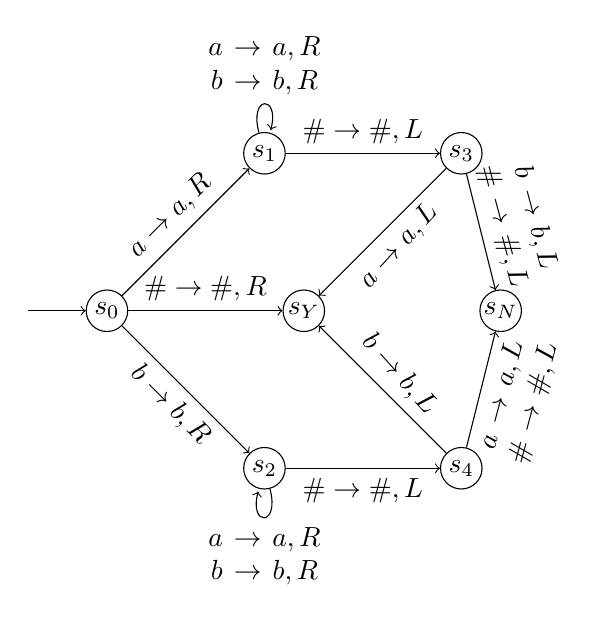
\begin{tikzpicture}
                \node[circle, draw=black, fill=white, inner sep=0pt, minimum size=15pt] (s0) at (0, 0) {$s_0$};
                \node[circle, draw=black, fill=white, inner sep=0pt, minimum size=15pt] (s1) at (2, 2) {$s_1$};
                \node[circle, draw=black, fill=white, inner sep=0pt, minimum size=15pt] (s2) at (2, -2) {$s_2$};
                \node[circle, draw=black, fill=white, inner sep=0pt, minimum size=15pt] (s3) at (4.5, 2) {$s_3$};
                \node[circle, draw=black, fill=white, inner sep=0pt, minimum size=15pt] (s4) at (4.5, -2) {$s_4$};
                \node[circle, draw=black, fill=white, inner sep=0pt, minimum size=15pt] (sY) at (2.5, 0) {$s_Y$};
                \node[circle, draw=black, fill=white, inner sep=0pt, minimum size=15pt] (sN) at (5, 0) {$s_N$};
                
                \draw[->] (-1, 0) -- (s0);
                \draw[->] (s0) -- node[above, rotate=45] {$a \to a, R$} (s1);
                \draw[->] (s0) -- node[below, rotate=-45] {$b \to b, R$} (s2);
                \draw[->] (s0) -- node[above] {$\# \to \#, R$} (sY);
                \draw[->] (s1) edge[loop above] node[above, text width=2cm, align=center] {$a \to a, R$ $b \to b, R$} (s1);
                \draw[->] (s2) edge[loop below] node[below, text width=2cm, align=center] {$a \to a, R$ $b \to b, R$} (s2);
                \draw[->] (s1) -- node[above] {$\# \to \#, L$} (s3);
                \draw[->] (s2) -- node[below] {$\# \to \#, L$} (s4);
                \draw[->] (s3) -- node[above, rotate=-75, text width=2cm, align=center] {$b \to b, L$ $\# \to \#, L$} (sN);
                \draw[->] (s4) -- node[below, rotate=75, text width=2cm, align=center] {$a \to a, L$ $\# \to \#, L$} (sN);
                \draw[->] (s3) -- node[below, rotate=48] {$a \to a, L$} (sY);
                \draw[->] (s4) -- node[above, rotate=-48] {$b \to b, L$} (sY);
            \end{tikzpicture}
            \caption{A Turing machine}
        \end{figure}
        \noindent Then, its corresponding TM program is:
\begin{lstlisting}[language=TML]
alphabet = {"a", "b"}
module startsAndEndsSame {
    switch tapehead {
        if blank {
            accept
        } if a {
            changeto a
            move right
            goto startsAndEndsSameMoveA
        } if b {
            changeto b
            move right
            goto startsAndEndsSameMoveB
        }
    }
}
module startsAndEndsSameMoveA {
    switch tapehead {
        while a {
            changeto a
            move right
        } while b {
            changeto b
            move right
        } if blank {
            changeto blank
            move left
            goto startsAndEndsSameCheckA
        }
    }
}
module startsAndEndsSameCheckA {
    switch tapehead {
        if a {
            changeto a
            move left
            accept
        } if b {
            changeto b
            move left
            reject
        } if blank {
            changeto blank
            move left
            reject
        }
    }
}
module startsAndEndsSameMoveB {
    switch tapehead {
        while a {
            changeto a
            move right
        } while b {
            changeto b
            move right
        } if blank {
            changeto blank
            move left
            goto startsAndEndsSameCheckB
        }
    }
}
module startsAndEndsSameCheckB {
    switch tapehead {
        if a {
            changeto a
            move left
            reject
        } if b {
            changeto b
            move left
            accept
        } if blank {
            changeto blank
            move left
            reject
        }
    }
}
\end{lstlisting}
    This is a complete program since TMs always include the required commands corresponding to \textit{if} and \textit{while} commands.
    \end{example}

    \begin{theorem} \label{thm:TM_to_TMP}
        Let $M$ be a TM, and let $P$ be the corresponding program for $M$. Then, $M$ and $P$ execute on every valid tape $T$ in the same way. That is, 
        \begin{itemize}
            \item for every valid index $n$, if we have tape $T_n$, tapehead index $i_n$ and module $m_n$ for the TM program $P$, and we have tape $S_n$, tapehead index $j_n$ and state $q_n$ for the TM $M$, then $T_n = S_n$, $i_n = j_n$ and $m_n$ is the corresponding module for $q_n$;
            \item $M$ terminates execution on $T$ if and only if $P$ terminates execution on $T$, with the same final status (\texttt{accept} or \texttt{reject}).
        \end{itemize}
    \end{theorem}
    \begin{proof}
        We prove this by induction. At the start, we have the same tape $T$ for both $M$ and $P$, with tapehead index $0$. Moreover, the first module in $P$ corresponds to the initial state $q_0$. So, the result is true if $n = 0$. Now, assume that the result is true for some integer $n$, where the TM state $q_n$ is not \texttt{accept} or \texttt{reject}. In that case, $T_n = S_n$, $i_n = j_n$ and $m_n$ is the corresponding module for $q_n$. Now, let $\sigma_n$ be the letter at index $i_n = j_n$ on the tape $T_n = S_n$. Compute $q(q_n, \sigma_n) = (q_{n+1}, \sigma_{n+1}, \texttt{dir})$. In that case,
        \[T_{n+1}(x) = \begin{cases}
            T_n(x) & x \neq i_n \\
            \sigma_{n+1} & \text{otherwise}
        \end{cases}, \qquad i_{n+1} = \begin{cases}
            i_n - 1 & \texttt{dir} = \texttt{left} \\
            i_n + 1 & \texttt{dir} = \texttt{right},
        \end{cases}\]
        and the next state is $q_{n+1}$. We know that the module $m_n$ in TM program $P$ corresponds to the state $q_n$, so it has a \texttt{changeto} $\sigma_{n+1}$ command for the case $\sigma_n$. In the case, the next tape for $P$ is:
        \[S_{n+1}(x) = \begin{cases}
            S_n(x) & x \neq i_n \\
            \sigma_{n+1} & \text{otherwise}.
        \end{cases}\]
        So, $T_{n+1} = S_{n+1}$. Similarly, the case also contains a \texttt{move dir} command. This implies that the next tapehead index for $P$ is:
        \[j_{n+1} = \begin{cases}
            j_n - 1 & \texttt{dir} = \texttt{left} \\
            j_n + 1 & \texttt{dir} = \texttt{right}.
        \end{cases}\]
        So, $i_{n+1} = j_{n+1}$. Now, if $q_{n+1} = q_n$, then the case block is a \textit{while} block, and vice versa. So, the next module to be executed is $m_n$. In that case, $m_{n+1}$ still corresponds to $q_{n+1}$. Otherwise, we have an \textit{if} block. In particular, if $q_{n+1}$ is the \texttt{accept} state, then the case for $\sigma_n$ contains the \textit{flow} command \texttt{accept}, and vice versa. In that case, execution terminates with the same final status of \texttt{accept}. The same is true for \texttt{reject}. Otherwise, the module contains the command \texttt{goto} $m_{n+1}$, where $m_{n+1}$ is the corresponding module for $q_{n+1}$. Therefore, if the result holds for $n$, it holds for $n+1$. Then, the result follows from induction.
    \end{proof}

    \begin{definition}
        Let $P$ be a complete TM program, and let $\Sigma$ be its alphabet. For each module $m$ in $P$, we define the \emph{corresponding state for $m$}, $q$ as follows- for each letter $\sigma$ in $\Sigma^+$, we define $\delta(q, \sigma) = (q', \sigma', \texttt{dir})$, where:
        \begin{itemize}
            \item the value $\sigma'$ is the letter given in the \textit{changeto} command within $m$;
            \item the value \texttt{dir} is the direction given in the \textit{move} command within $m$;
            \item if the \textit{flow} command in $m$ is \texttt{accept}, then $q'$ is the \texttt{accept} state; if it is \texttt{reject}, then $q'$ is the \texttt{reject} state; otherwise, $q'$ is the state corresponding to the module given in the \textit{goto} command within $m$.
        \end{itemize}
        Then, the TM with all the states $q$, alphabet $\Sigma$, the transition function $\delta$ and initial state $q_0$ corresponding to the first module in $P$ is called the \emph{corresponding TM for $P$}.
    \end{definition}

    \begin{example}
        Consider the following complete TM program:
\begin{lstlisting}[language=TML]
alphabet = {"a", "b"}
module moveToEnd {
    switch tapehead {
        while a {
            changeto a
            move right
        } while b {
            changeto b
            move right
        } if blank {
            changeto blank
            move left
            goto checkAFirst
        }
    }
}
module checkAFirst {
    switch tapehead {
        if a {
            changeto blank
            move left
            goto checkASecond
        } if b, blank {
            changeto blank
            move left
            reject
        }
    }
}
module checkASecond {
    switch tapehead {
        if a {
            changeto blank
            move left
            accept
        } if b, blank {
            changeto blank
            move left
            reject
        }
    }
}
\end{lstlisting}
    Then, its corresponding TM is the following:
    \begin{figure}[H]
        \centering
        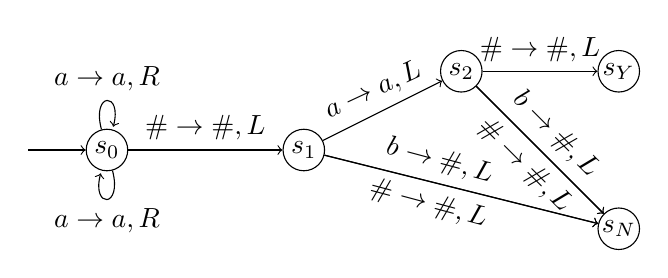
\begin{tikzpicture}
            \node[circle, draw=black, fill=white, inner sep=0pt, minimum size=15pt] (s0) at (-0.5, 0) {$s_0$};
            \node[circle, draw=black, fill=white, inner sep=0pt, minimum size=15pt] (s1) at (2, 0) {$s_1$};
            \node[circle, draw=black, fill=white, inner sep=0pt, minimum size=15pt] (s2) at (4, 1) {$s_2$};
            \node[circle, draw=black, fill=white, inner sep=0pt, minimum size=15pt] (sY) at (6, 1) {$s_Y$};
            \node[circle, draw=black, fill=white, inner sep=0pt, minimum size=15pt] (sN) at (6, -1) {$s_N$};
            
            \draw[->] (-1.5, 0) -- (s0);
            \draw[->] (s0) edge[loop above] node {$a \to a, R$} (s0);
            \draw[->] (s0) edge[loop below] node {$a \to a, R$} (s0);
            \draw[->] (s0) -- node[above] {$\# \to \#, L$} (s1);

            \draw[->] (s1) -- node[above, rotate=25] {$a \to a, L$} (s2);
            \draw[->] (s1) -- node[below, rotate=-15, pos=0.4] {$\# \to \#, L$} (sN);
            \draw[->] (s1) -- node[above, rotate=-15, pos=0.4] {$b \to \#, L$} (sN);

            \draw[->] (s2) -- node[above] {$\# \to \#, L$} (sY);

            \draw[->] (s2) -- node[above, rotate=-45] {$b \to \#, L$} (sN);
            \draw[->] (s2) -- node[below, rotate=-45] {$\# \to \#, L$} (sN);
        \end{tikzpicture}
        \caption{The TM corresponding to the program above. The state $s_0$ corresponds to the module \texttt{moveToEnd}; the state $s_1$ corresponds to the module \texttt{checkAFirst}; and the state $s_2$ corresponds to the module \texttt{checkASecond}.}
    \end{figure}
    \end{example}

    \begin{theorem} \label{thm:TMP_to_TM}
        Let $P$ be a complete TM program, and let $M$ be the corresponding TM for $P$.  Then, $P$ and $M$ execute on every valid tape $T$ in the same way. That is,
        \begin{itemize}
            \item for every valid index $n$, if we have tape $T_n$, tapehead index $i_n$ and module $m_n$ for TM program $P$, and we have tape $S_n$, tapehead index $j_n$ and state $q_n$ for the TM $M$, then $T_n = S_n$, $i_n = j_n$ and $q_n$ is the corresponding state for $m_n$;
            \item $P$ terminates execution on $T$ if and only if $M$ terminates execution on $T$, with the same final status (\texttt{accept} or \texttt{reject}).
        \end{itemize}
    \end{theorem}
    \begin{proof}
        We prove this by induction as well. At the start, we have the same tape $T$ for both $P$ and $M$, with tapehead index $0$. Moreover, the initial state $q_0$ in $M$ corresponds to the first module in $P$. So, the result is true if $n = 0$. Now, assume that the result is true for some integer $n$, which is not the terminating step in execution. In that case, $S_n = T_n$, $j_n = i_n$ and $q_n$ is the corresponding state for $m_n$. Now, let $\sigma_n$ be the letter at index $j_n = i_n$ on the tape $S_n = T_n$. If the block in $m_n$ corresponding to $\sigma_n$ is a \textit{while} block, then we know that its body is partially complete, and so is composed of the following commands:
        \begin{itemize}
            \item \texttt{changeto} $\sigma_{n+1}$
            \item \texttt{move dir}
        \end{itemize}
        So, we have $\delta(q_n, \sigma_n) = (q_n, \sigma_{n+1}, \texttt{dir})$. Using the same argument as in \textbf{\ref{thm:TM_to_TMP}}, we find that $T_{n+1} = S_{n+1}$ and $i_{n+1} = j_{n+1}$. Also, $q_{n+1} = q_n$ is the corresponding state for $m_{n+1} = m_n$. Otherwise, we have an \textit{if} command. In this case, the case body is complete, and so composed of the following commands:
        \begin{itemize}
            \item \texttt{changeto} $\sigma_{n+1}$
            \item \texttt{move dir}
            \item \texttt{accept}, \texttt{reject} or \texttt{goto} $m_{n+1}$.
        \end{itemize}
        So, we have $\delta(q_n, \sigma_n) = (q_n, \sigma_{n+1}, \texttt{dir})$, where $\sigma_{n+1}$ is the corresponding state to the \textit{flow} command present. Here too, we have $T_{n+1} = S_{n+1}$, $i_{n+1} = j_{n+1}$. If we have an \texttt{accept} command in the body, then $q_{n+1}$ is the accepting state, and vice versa. So, we terminate execution with the final status of \texttt{accept}. The same is true for \texttt{reject}. Otherwise, the state $q_{n+1}$ is the corresponding state to the module $m_{n+1}$. So, the result follows from induction.
    \end{proof}

    \section{Valid to complete programs}
    \begin{definition}
        Let $P$ be a TM program. We define the TM program $P_1$ to be the \emph{first completion of $P$} as follows:
        \begin{itemize}
            \item the alphabet of $P_1$ is the same as the alphabet of $P$;
            \item for every block $b$ in every module $m$ of $P$, $P_1$ has a module with body the block $b$. If the block is not the final block in $m$, it has an additional flow command to the next block in the module. The order of the modules is the same as the order of the original blocks.
        \end{itemize}
        We define the TM program $P_2$ to be the \emph{second completion of $P$} as follows:
        \begin{itemize}
            \item the alphabet of $P_2$ is the same as the alphabet of $P$;
            \item for every module $m$ of $P$ with a \textit{basic} block, replace it with a \textit{switch} block where every case is an \textit{if} command with body the original basic block.
        \end{itemize}
        Finally, we define the TM program $P^+$ to be the \emph{(third) completion of $P$} as follows:
        \begin{itemize}
            \item the alphabet of $P^+$ is the same as the alphabet of $P$;
            \item for every non-complete module $m$ of $P$, replace it with a complete block by adding the default commands:
            \begin{itemize}
                \item if the \textit{changeto} command is missing, add the \textit{changeto} command corresponding to the case value;
                \item if the \textit{move} command is missing, add the command \texttt{move left};
                \item if the \textit{flow} command is missing, add the command \texttt{reject}.
            \end{itemize}
        \end{itemize}
    \end{definition}

    \begin{remark}
        For any TM program $P$, its completion $P^+$ is complete by construction.
    \end{remark}

    \begin{remark}
        Let $P$ be a TM program. For every block $b$ in $P$, there is a complete module $m$ in the completion program $P^+$. We say that $m$ is the \emph{corresponding complete module} of $b$.
    \end{remark}
    
    \begin{example}
        Consider the following TM program:
\begin{lstlisting}[language=TML]
alphabet = {"a", "b"}
module simpleProgram {
    changeto b
    move left
    move right
    accept
}
\end{lstlisting}
\noindent Them, its first completion is the following program:
\begin{lstlisting}[language=TML]
alphabet = {"a", "b"}
module simple1 {
    changeto b
    move left
    goto simple2
}
module simple2 {
    move right
    accept
}
\end{lstlisting}
\noindent The second completion is the following program:
\begin{lstlisting}[language=TML]
alphabet = {"a", "b"}
module simple1 {
    switch tapehead {
        if a, b, blank {
            changeto b
            move left
            goto simple2
        }
    }
}
module simple2 {
    switch tapehead {
        if a, b, blank {
            move right
            accept
        }
    }
}
\end{lstlisting}
\noindent Finally, the completion of $P$ is the following:
\begin{lstlisting}[language=TML]
alphabet = {"a", "b"}
module simple1 {
    switch tapehead {
        if a {
            changeto b
            move left
            goto simple2
        } if b {
            changeto b
            move left
            goto simple2
        } if blank {
            changeto b
            move left
            goto simple2
        }
    }
}
module simple2 {
    switch tapehead {
        if a {
            changeto a
            move right
            accept
        } if b {
            changeto b
            move right
            accept
        } if blank {
            move right
            accept
        }
    }
}
\end{lstlisting}
    \end{example}

    \begin{theorem}
        Let $P$ be a valid TM program. Then, $P$ and its completion $P^+$ execute on every valid tape $T$ in the same way. That is,
        \begin{itemize}
            \item for every valid index $n$, if we have tape $T_n$, tapehead index $i_n$ and module $m_n$ with executing block $b_n$ for the TM program $P$, and we have tape $S_n$, tapehead index $j_n$ and module $t_n$, then $T_n = S_n$, $i_n = j_n$, and $t_n$ is the corresponding complete module block of $b_n$;
            \item $P$ terminates execution on $T$ if and only if $P^+$ terminates execution on $T$, with the same final status (\texttt{accept} or \texttt{reject}).
        \end{itemize}
    \end{theorem}
    \begin{proof}
        We prove this by induction. At the start, we have the same tape $T$ for both $P$ and $P^+$, with tapehead index 0. Moreover, the corresponding (complete) module of the first block in the first module of $P$ is the first module of $P$. So, the result is true if $n = 0$. Now, assume that the result is true for some integer $n$, where the block $b_n$ in the TM program $P$ does not end with a terminating \textit{flow} command. Let $\sigma_n$ be the letter at index $i_n = j_n$ on the tape $S_n = T_n$.
        
        If the \textit{changeto} command is missing in $b_n$ for $\sigma_n$, then the next tape $T_{n+1} = T_n$. In the complete module $m_n$, the case for $\sigma_n$ will have \texttt{changeto} $\sigma_n$. So, the next tape is given by:
        \[S_{n+1}(x) = \begin{cases}
            S_n(x) & x \neq j \\
            \sigma_n & \text{otherwise}
        \end{cases}.\]
        Therefore, we have $S_{n+1} = S_n$ as well. So, $T_{n+1} = S_{n+1}$. Otherwise, we have the same \textit{changeto} command, in which case $T_{n+1} = S_{n+1}$ as well.

        If the \textit{move} command is missing in $b_n$ for $\sigma_n$, then the next tapehead index $i_{n+1} = i_n - 1$. In the complete module $m_n$, the case for $\sigma_n$ will have \texttt{move left}, so we also have $j_{n+1} = j_n - 1$. So, we have $i_{n+1} = j_{n+1}$. Otherwise, we have the same \textit{move} command, meaning that $i_{n+1} = j_{n+1}$.

        If the block $b_n$ is a \textit{switch} block with a \textit{while} case for $\sigma_n$, then this is still true in the module $m_n$. So, the next block to be executed in $P$ is $b_n$, and the next module to be executed in $P^+$ is $m_n$. In that case, the corresponding module of the block $b_{n+1} = b_n$ is still $m_{n+1} = m_n$. Instead, if the block $b_n$ has no \textit{flow} command for $\sigma_n$, and is not the last block, then the next block to execute is the block just below $b_n$, referred as $b_{n+1}$. By the definition of $P^+$, we find that the case block in the module $m_n$ has a \textit{goto} command, going to the module $m_{n+1}$ which corresponds to the block $b_{n+1}$. Also, if the \textit{flow} command is missing for $\sigma_n$ and this is the last block, then execution is terminated with the status \texttt{reject} for the program $P$. In that case, the case for $\sigma_n$ in the module $m_n$ has the \texttt{reject} command present, so the same happens for $P^+$ as well. Otherwise, both $P$ and $P^+$ have the same flow command, meaning that there is either correspondence between the next block and the next module, or both the program terminate with the same status.
    \end{proof}
\end{document}